\documentclass[acmsmall, nonacm]{acmart}


\renewcommand\footnotetextcopyrightpermission[1]{} % removes footnote with conference information in first column
\makeatletter
\let\@authorsaddresses\@empty % removes authors' addresses from first page footer
\makeatother

\usepackage[linesnumbered,ruled,vlined]{algorithm2e}
\usepackage{tikz}
\usetikzlibrary{positioning}
\usepackage{xcolor}
\definecolor{mygreen}{RGB}{0,120,0}
\usepackage{wrapfig}
\usepackage{capt-of}
\usepackage{syntax}
\usepackage{graphicx}

%% (Not sure if this is needed)
%% \BibTeX command to typeset BibTeX logo in the docs
\AtBeginDocument{%
  \providecommand\BibTeX{{%
    \normalfont B\kern-0.5em{\scshape i\kern-0.25em b}\kern-0.8em\TeX}}}


\begin{document}


\title{A Divide-and-Conquer Approach to Discovering Minimal Realizable Grammars}


\author{Will Thomas}
\author{Logan Schmalz}
\author{Sarah Johnson}


\maketitle

\section{Introduction}
%%(Presents the central idea of your project and summarizes the takeaways)

\section{Background}
Our project is based on the work of Semantic-Guided Synthesis (SemGuS) \cite{semgus}. SemGuS aims to be ``a language-agnostic logic-based framework for program synthesis problems over arbitrary semantics''. A SemGuS problem is defined by language syntax given as a Regular Tree Grammar (RTG), language semantics given as Constrained Horn Clauses (CHCs), and problem specification given by logical constraints or input-output examples. The feature that sets SemGuS apart from Syntax-Guided Synthesis (SyGuS) is the ability to define a custom semantics for a language, as SyGuS cannot express problems that contain semantics outside of supported theory. SemGuS accepts recursively defined big-step semantics allowing synthesis over imperative programming languages that contain loops with unbounded behaviour. Kim et al. not only designed the SemGuS framework but also developed an algorithm for solving SemGuS problems. The algorithm encodes SemGuS problems as a proof search over CHCs and is capable of both synthesizing programs and proving unrealizability, the latter of which our project relies on.


\section{Overview}
%%(Gives step by step working of your project on a single example)

\begin{wrapfigure}{r}{8.1cm}
  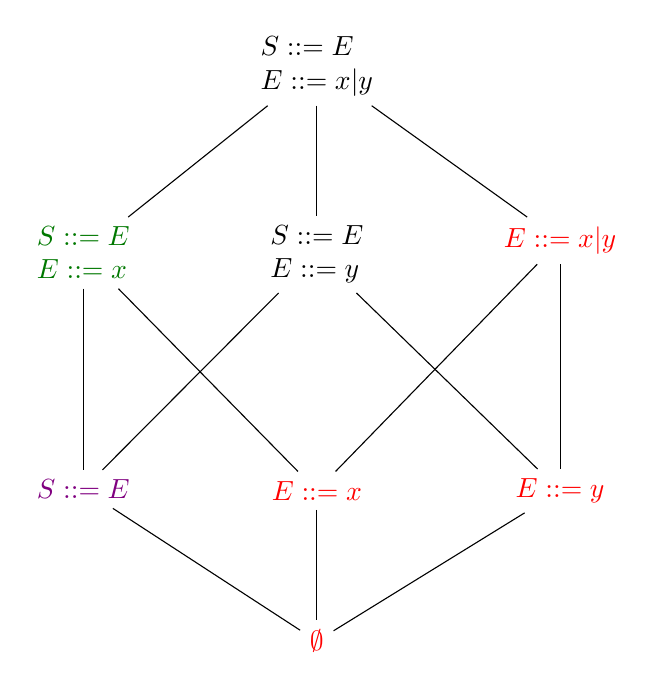
\begin{tikzpicture}[node distance=3cm]
    \title{lattice 2}
    \node(123)      [align=left]              {$S ::= E$ \\ $E ::= x \text{ }\vert\text{ } y$};
    \node(12)       [below left=2cm of 123, align=left] {$\color{mygreen} S ::= E$ \\ $\color{mygreen} E ::= x$};
    \node(13)      [below=1.4cm of 123, align=left]  {$S ::= E$ \\ $E ::= y$};
    \node(23)      [below right=2cm of 123, align=left]       {$\color{red} E ::= x \text{ }\vert\text{ } y$};
    \node(1)      [below of=12]       {$\color{violet} S ::= E$};
    \node(2)      [below of=13]       {$\color{red} E ::= x$};
    \node(3)      [below=2.6cm of 23]       {$\color{red} E ::= y$};
    \node(empty)      [below=1.4cm of 2]       {$\color{red} \emptyset$};

    \draw(123)       -- (12);
    \draw(123)       -- (13);
    \draw(123)       -- (23);
    \draw(12)       -- (1);
    \draw(12)       -- (2);
    \draw(13)      -- (1);
    \draw(13)      --  (3);
    \draw(23)      --  (2);
    \draw(23)      --  (3);
    \draw(1)      --  (empty);
    \draw(2)      --  (empty);
    \draw(3)      --  (empty);
  \end{tikzpicture}
  \captionof{figure}{Subgrammar Lattice}
  \label{fig:lattice}
\end{wrapfigure}

Consider a very simple example problem: synthesize a function that returns the first projection of an ordered pair. Our goal is to find a minimal realizable subgrammar for this problem. The full grammar consists of a start nonterminal symbol $S$ with a single production rule $E$. $E$ is an expression nonterminal symbol with two production rules $x$ and $y$. $x$ returns the first parameter given to the function while $y$ returns the second. In this example, it is obvious to see that $y$ can be removed from the language and the problem is still realizable.

In our work, we design a sound and complete algorithm for finding a minimal realizable subgrammar. Given some grammar, the algorithm generates every subgrammar (including invalid ones) and checks realizability under each one. The total set of subrammars is equal to the power set of the production rules and forms a lattice under the subset relation as shown in Figure \ref{fig:lattice}. The red text denotes invalid grammars due to missing start symbol; the purple text denotes invalid grammars due to missing nonterminal symbol; and the green text denotes the minimal realizable grammar given the behavioural specification.


\section{Technical Details}

At its core, our approach had two modes that it could take.
We could either remove Non-Terminals from the grammar, or
specific production rules related to a Non-Terminal.
These approaches, their benefits and limitations will
be explored further in the next two subsections.
Throughout both examples, we will keep in mind the general purpose grammar
presented in Figure~\ref{fig:Technical-Grammar}.


\begin{figure}[ht]
  \centering
  \resizebox{0.75\textwidth}{!}{
    \begin{tabular}{ccccc}
      $\langle G_1 \rangle$ & ::= & $\alpha_{G_{1,1}}$ & $| \ldots |$ & $\alpha_{G_{1,M_1}}$ \\
      $\langle G_2 \rangle$ & ::= & $\alpha_{G_{2,1}}$ & $| \ldots |$ & $\alpha_{G_{2,M_2}}$ \\
      \vdots                &     & \vdots             &              & \vdots               \\
      $\langle G_N \rangle$ & ::= & $\alpha_{G_{N,1}}$ & $| \ldots |$ & $\alpha_{G_{N,M_N}}$ \\
    \end{tabular}
  }
  \caption{Example Technical Grammar $G$}
  \Description{Example technical grammar non terminals and production rules}
  \label{fig:Technical-Grammar}
\end{figure}

Additionally, the general purpose algorithm presented in Figure~\ref{fig:Algorithm} is the approach that will be taken for both
the Non-Terminal and the Production Rule modes.

\begin{figure}[H]
  \begin{algorithm}[H]
    \KwIn{l : List[SpecEvents]}
    \KwOut{l' : Option[List[SMTCommand]]}
    \SetAlgoLined

    var $declT, defT, hornC, constrs, synthFun$ = l.filter(classTypeFilter())

    var $requiredEvs$ = $constrs ::: synthFun$

    var $combinedEvs$ = $defT ::: hornC$

    \BlankLine
    \For{$i \leftarrow 1\ \KwTo\ length(combinedEvs)$}{
      \For{$part \in combinedEvs.combinations(i)$}{
        var $smtEncoding$ = $semgus2SMT(part ::: requiredEvs)$

        \If{$checkSat(smtEncoding)$}{
          \Return{Some($smtEncoding$)}
        }
      }
    }
    Otherwise we return None;

    \caption{Minimal Sub-Grammar}
  \end{algorithm}
  \caption{General Purpose Realizability Algorithm}
  \label{fig:Algorithm}
  \Description{Basic psuedo code for the general purpose algorithm}
\end{figure}

The key features of this algorithm are first splitting the problem based upon the 
type of the ``SpecEvents'' that are used. In particular, all realizability problems will need to incorporate the constraints and the synthesize function events. Based upon the mode of the algorithm, we will either
choose from partitions of the events (the partitions have grouped together the non-terminals with all of their production rules) or choose from all events (for production rule mode).
From then, the baseline Messy method for translating a list of spec events into an SMT encoding (as Constrained Horn Clauses) is used. We then check SAT on the output from Messy and return realizable if SAT, or continue if UNSAT.

\subsection{Combinatoric Complexity}
One important pre-requisite to understanding the design decisions made for this project is understanding the computational complexity of a combinatoric problem, such as the one we are attempting.
While the individual times to compute realizability or unrealizability may be
relatively quick, the number of times we have to compute it due to
generating grammar combinations is immense.
In particular, we must (in the worst case) generate $2^N$ sub-grammars to
remain a decision procedure for realizability.
$$\sum_{i = 0}^{N} {N \choose x} == 2^N$$
Ultimately, understanding the inherently exponential nature of the problem
we must solve will help provide a background on why different modes were created
and why optimization may be required for a true implementation to excel.


\subsection{Non-Terminal Mode}
In this mode, we would remove whole Non-Terminals from the grammar at a time.
This is in essence a very coarse grained approach to finding a minimal
realizable sub-grammar. Given the example grammar $G$ from Figure~\ref{fig:Technical-Grammar}, it can be seen that there are $N$ non-terminals in
that grammar.
Our approach for non-terminal mode will be to start enumerating all combinations
of the non-terminals in grammar $G$. We will start this enumeration from the bottom-up, as the time to process a small grammar and decide either
realizability or unrealizability will be minimal. This way if a small grammar
is realizable, we can quickly dispatch it to a state-of-the-art synthesis tool
for complete synthesis. The downfall of our technique is that by enumerating from the bottom-up of for sub-grammars, if a grammar is only realizable with the majority (or in the worst case all) non-terminals it will take a long time to complete.

One thing that the reader may be considering is that the removal of a non-terminal will violate the ``minimal'' property of our algorithm. This is technically true, as the output grammar will not contain the least number of both non-terminals and production rules required to complete its synthesis task, but when viewed from the realm of non-terminals it remains true. The non-terminal mode of the algorithm will be guaranteed to yield a sub-grammar with the ``minimal'' number of non-terminals required for completing the task.

\subsection{Production Rule Mode}
The general approach in Production Rule mode is quite similar to the Non-Terminal mode described above. The key difference is that instead of grouping together non-terminals and their corresponding production rules, we just remove production rules. Production rule mode can be thought of as a more extreme version of the non-terminal mode: the strengths are improved, but the weaknesses also worsened.
If a small realizable sub-grammar exists, Production rule mode is bound to find it quickly and allow for a vast deal of improved synthesis time as the grammar the synthesizer must operate over is quite small. In the case that the problem is not realizable, even with a full grammar, then the time it takes for production rule mode to complete will be $2^K$, where $K = \sum_{i = 1}^{N} M_i$ (recall $N,M$ for the example grammar in Fig~\ref{fig:Technical-Grammar}).
Depending on the size of the grammar, and the amount of production rules required
to solve a given synthesis problem, this mode could be highly beneficial or a complete waste of time.

\section{Implementation}
%%(The general technical ideas are never enough to get a working implementation :) You probably had to cut corners, optimize certain things to make it practical, etc. which go here)

\section{Evaluation}

In this section, we will dive into our evaluation, comparing the run time of the original Messy solver to our NT (Non-Terminal) mode. We did not collect data on the running of Prod (Production Rule) mode as the time for each benchmark to complete in Prod mode was extremely long and would establishing a good dataset was infeasible due to time constraints.

\begin{figure}[H]
  \centering
  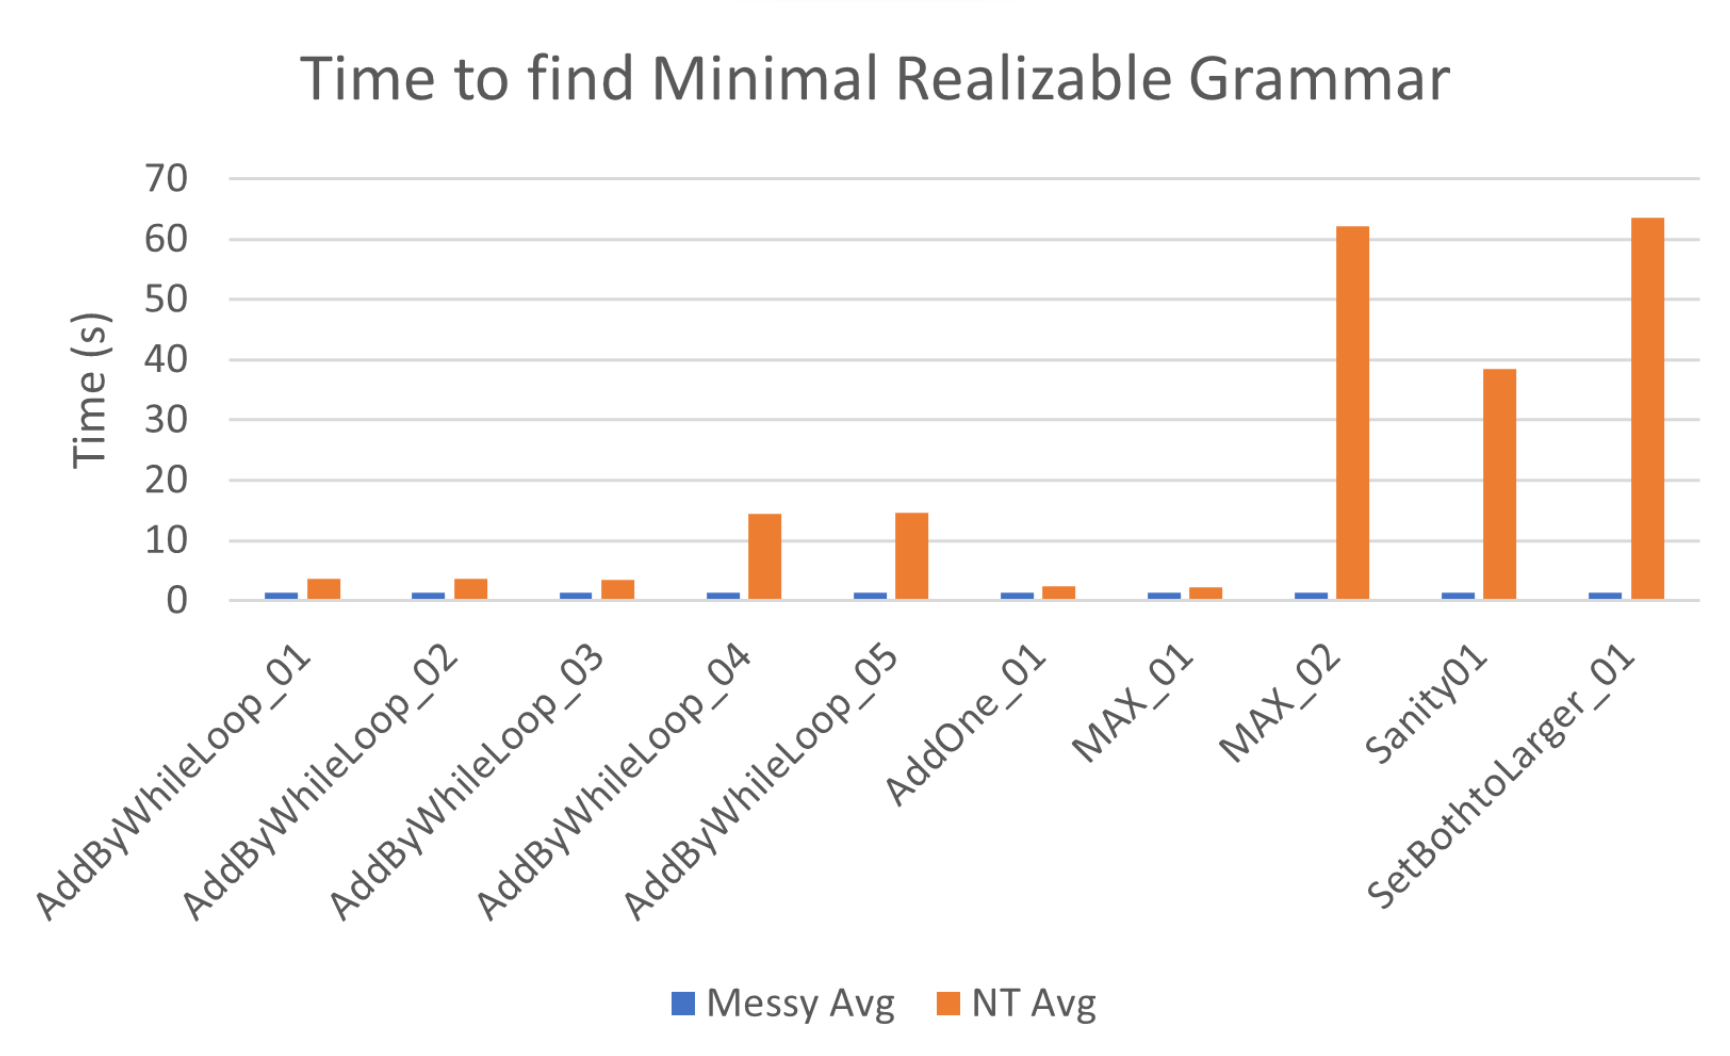
\includegraphics[width=1\textwidth]{Results.png}
  \caption{Benchmarking Results}
  \label{fig:Benchmarking-Results}
  \Description{Benchmarking results for time to run vs technique}
\end{figure}

Unfortunately, both our NT and Prod approaches are slower than the original Messy Solver on all benchmarks.
Additionally, our approach was limited in exactly the same ways as the the original Messy solver. For one, it cannot parse SemGuS files that Messy cannot, of which a surprising number of the Messy benchmarks were actually un-parseable.
We had to invalidate 8 tests from the 18 “Messy benchmarks” due to the fact that Messy itself could not parse them to even attempt solving.

One great benefit however was our Prod approach was able to discover a minimal sub-grammar that was smaller than the full grammar. For the test AddByWhileLoop_1 (notably the only problem we ran Prod on to completion), we
generated a grammar in 434 seconds that used 11 less variables, 2 less relations, and 7 less semantic rules, but was still realizable.
This reduction implies that we are able to get rid of certain production rules, but not the non-terminals related to those production rules, since
the NT mode was not able to find a minimal sub-grammar for the same test.
However, this comes at a very high cost, as the time it took our solver to find the minimal realizable grammar was more than $100 \times$ that of the original Messy solver. Further testing would be required to determine if the time saved during synthesis by using this smaller sub-grammar is worth the upfront cost of Prod mode.

\section{Future Work}
%%(Potential future work that you think could be interesting)

\section{Conclusion}
%%(Your concluding take on the project and learnings)

\bibliographystyle{ACM-Reference-Format}
\bibliography{projectrefs}


\end{document}

